%====================================================================================
% Preamble
%------------------------------------------------------------------------------------

\documentclass{beamer}

% Essential Packages
% Apartado de letras
\usepackage[utf8]{inputenc}
\usepackage[T1]{fontenc}
\usepackage[spanish]{babel}

% Aparatdo matemático
\usepackage{amsmath}
\usepackage{amsfonts}
\usepackage{amssymb}
\usepackage{mathtools}

% Apartado tablas, figuras, y otros
\usepackage{multirow,booktabs,setspace,caption,multicol,tabularx, tabulary}
\captionsetup{skip=0pt}

% Apartado Tablas y Figuras en APA
\DeclareCaptionLabelSeparator*{spaced}{\\[1ex]}
\captionsetup[table]{name = Tabla, textfont=it,format=plain,justification=justified,
	singlelinecheck=false,labelsep=spaced,skip=0pt}
\captionsetup[figure]{name = Figura, labelsep=period,labelfont=it,justification=justified,
	singlelinecheck=false,font=doublespacing}
	% Para hacer tablas APA más fácil
	\usepackage[flushleft]{threeparttable}

% Apartado hyperres
\usepackage{hyperref}

% Apartado Tikz
\usepackage{tikz, pgfplots}
\usetikzlibrary{positioning,calc,arrows}
\usetikzlibrary{shapes.arrows}
\usetikzlibrary{patterns}

	\tikzset{ % to make dots on the graph
		dot/.style = {circle, fill, minimum size=#1,
			inner sep=0pt, outer sep=0pt},
		dot/.default = 6pt % size of the circle diameter 
	}

% Apartado de colores
\usepackage{xcolor}

% Apartado tipò de letra
\usepackage{textcomp}
\usepackage{libertine}
\usepackage[libertine]{newtxmath}

% Apartado de íconos
\usepackage{fontawesome5}

%Creación de entornos matemáticas
\newtheorem{defi}{Definición}[section]
\newtheorem{lema}{Lema}[section]
\newtheorem{teo}{Teorema}[section]
\newtheorem{coro}{Corolario}[section]

% Diversos
\usefonttheme[onlymath]{serif}
\usepackage{remreset}
\usepackage{makecell}
\usepackage{float}
\usepackage{subfigure}

% Apartado justificación de textos
\usepackage{ragged2e}
\justifying
\renewcommand{\raggedright}{\leftskip=0pt \rightskip=0pt plus 0cm}

% Apartado de configuración del Beamer
\mode<presentation> {
	\usetheme{Frankfurt}
	\setbeameroption{show notes}
	\setbeamertemplate{footline}[frame number]
	\usefonttheme[onlylarge]{structuresmallcapsserif}
	\usefonttheme[onlysmall]{structurebold}
	\usecolortheme{beaver}
	\setbeamercovered{transparent}
	\setbeamertemplate{navigation symbols}{}
	
	\setbeamercolor{section in head/foot}{bg=gray!8!white,fg=yellow!25!red}	
	\setbeamercolor{frametitle}{bg=gray!15!white,fg=yellow!20!red}
	\setbeamercolor{title}{bg=gray!25!white,fg=yellow!20!red}
	\setbeamercolor{item projected}{fg=white,bg=yellow!30!red}
}

% Apartado transparencia de contenido
\AtBeginSection[]
{
	\begin{frame}<beamer>{Contenido}
		\tableofcontents[currentsection,currentsubsection]
	\end{frame}
}
\AtBeginSubsection[]
{
	\begin{frame}<beamer>{Contenido}
		\tableofcontents[currentsection,currentsubsection]
	\end{frame}
}

% Apartado de logo
\logo{
\includegraphics[scale=.06]{figures/logo.png}}

% Apartado cambio como por punto
\decimalpoint

%====================================================================================

%====================================================================================
% Body
%====================================================================================
% Title Page
%-----------
\title{Teoría Microeconómica II\\
		Tema 2: COMPLETAR}
\author[José A. Valderrama]{\large{José A. Valderrama}\\
		{\small \texttt{jvalder@ulima.edu.pe} {\color{black}{\faIcon{envelope}}}}}
\institute{\large Universidad de Lima - Carrera de Economía}

\date{\today}

%------------------------------------------------------------------------------------
% Title
%---------
\begin{document}
	\begin{frame}[plain]
		\maketitle
	\end{frame}
%------------------------------------------------------------------------------------
% Sections
%---------
	\begin{frame}{Contenido}
		\tableofcontents
	\end{frame}

%1) Producción en la caja de Edgeworth------------
	%====================================================================================
\section{Introducción}
%====================================================================================

\begin{frame}{Introducción}
	La selección adversa es un problema en que las partes contratantes no se conocen a la perfección.\\[0.3cm]
	
	Aparece cuando el agente tiene más información sobre alguna de las variables relevantes para la relación\\[0.3cm]
	
	Quien posee ventaja informativa sobre un tercero puede tener interés para ocultarla o usarla para su propio beneficio\\[0.3cm]
	
	Consecuencias:
		\begin{itemize}
			\item modificaciones en el equilibrio de mercado
			\item Inexistencia de equilibrio.
		\end{itemize}
\end{frame}
%2) La frontera de posibilidades de producción----
	%====================================================================================
\section[Akerlof]{El mercado de autos usados (artículo de Akerlof}
%====================================================================================

\begin{frame}{El artículo de Akerlof}
	Fue el primero que introdujo el concepto de información asimétrica\\[0.3cm]
	Su argumento básico es que en muchos mercados el comprador emplea alguna estadística del mercado para medir el valor de una clase de bienes\\[0.3cm]
	Entonces , el comprador mira el promedio del mercado completo mientras el vendedor tiene más conocimiento privado de un aspecto específico\\[0.3cm]
	Según Akerlof esta información asimétrica le da al vendedor un incentivo para vender bienes por debajo de la calidad media del mercado\\[0.3cm]
	
\end{frame}
%------------------------------------------------
\begin{frame}{El artículo de Akerlof}
	Entonces , la calidad promedio de los bienes en el mercado se reducirá con el tamaño del mercado\\[0.3cm]
	Tales diferencias en retornos sociales y privados puede ser mitigado por un número de diferentes instituciones del mercado\\[0.3cm]
	Akerlof empieza asumiendo un modelo del mercado de automóviles , donde hay cuatro tipos de autos:
		\begin{itemize}
			\item Hay autos nuevos y autos viejos ,
			\item En cada uno , pueden ser autos buenos o malos
			\item Los autos malos son popularmente conocidos como ``limones'' en EEUU.
		\end{itemize}

\end{frame}
%------------------------------------------------
\begin{frame}{El artículo de Akerlof}
	Existen dos tipos de agentes: Compradores y Vendedores
		\begin{enumerate}
			\item Compradores
				\begin{itemize}
					\item Función de utilidad: $U_v = M +1.5qn$
						\begin{itemize}
							\item $M$ = Consumo de otros bienes
							\item $q$ = Calidad del auto
							\item $n$ = $\left\lbrace 0,1\right\rbrace $ 1 compra auto, 0 no compra
						\end{itemize}
					\item Restricción presupuestaria: $y_v = M + pn$
						\begin{itemize}
							\item $y_c$ = Ingreso
							\item $p$ = Precio del auto
						\end{itemize}
				\end{itemize}
			La calidad del auto $(q)$ es información privada del vendedor. El comprador aprecia $``q''$ como la calidad media del mercado, mientras que el vendedor distingue la de cada auto
		\end{enumerate}
\end{frame}
%------------------------------------------------
\begin{frame}{El artículo de Akerlof}
	Dada la incertidumbre de $``q''$ el comprador maximiza su utilidad esperada:
		\begin{itemize}
			\item $E(U_c)=M+1.5E(q)n \quad E(q) = \mu =$ Calidad media observada
		\end{itemize}
	Sustituyendo $M$ de la $r.p .$ $\longrightarrow M =y_c - pn$ 
		\begin{itemize}
			\item $E(U_c) = y_c - pn + 1.5\mu n \longrightarrow $  factor común a ``$n$''
			\item $E[U_c] = y_c +\left[ 1.5\mu - p\right]n$
		\end{itemize}
	Decisión:
		\begin{itemize}
			\item $n=1$ compra si percibe la calidad del auto por encima del precio; es decir, si $1.5\mu \geq p$
			\item $n=0$ no compra si percibe la calidad del auto por encima del precio; es decir, si $1.5\mu \leq p$
		\end{itemize}
\end{frame}
%------------------------------------------------
\begin{frame}{El artículo de Akerlof}
	\begin{enumerate}[2]
		\item Vendedores
			\begin{itemize}
				\item Función de utilidad:$U_v = M +qn$
				\item Restricción presupuestaria: $y_v = M + pn$
				\item $n=1$ mantener el auto, $n=0$ vender del auto
			\end{itemize}
		Por tanto:
			\begin{itemize}
				\item Para el vendedor la $U_{MG} = q$
				\item Para el comprador la $U_{MG} = 1.5q$
			\end{itemize}
		Esto es lo que garantiza potenciales ganancias en el intercambio.
	\end{enumerate}
\end{frame}
%------------------------------------------------
\begin{frame}{El artículo de Akerlof}
	El vendedor conoce $q$
		\begin{itemize}
			\item Sustituyendo $M$ de la $r.p.$ donde $M=y_v - pn$
			\item $U_v = y_v - pn +qn \longrightarrow $factor común a ``$n$''
			\item $U_v = y_v + (q-p)n$
		\end{itemize}
	Decisión
		\begin{itemize}
			\item $n = 0$ vende si $p\geq p$ (Precios $\geq$ Calidad)
			\item $n = $ vende si $p\leq p$ (Precios $\leq$ Calidad)
		\end{itemize}
	¿Cómo se forma $\mu$
\end{frame}
%------------------------------------------------
\begin{frame}{El artículo de Akerlof}
	Akerlof partió del supuesto simplificador que la calidad de los autos se distribuye de manera uniforme en el rango $[0,2]$, por tanto $f(q)= 1/2$\\[0.3cm]
	
	La oferta de autos es $S=(1/2)pN$ porque:
		\begin{itemize}
			\item la probabilidad de vender es $(1/2)p$
			\item Número de autos usados $()N$
		\end{itemize}
	Es decir, la oferta es el número de autos usados por la probabilidad de venta. Tenemos todos los datos necesarios para calcular el equilibrio de esta economía
		\begin{itemize}
			\item Demanda: $(3/2) \mu \geq p$
			\item Oferta:$(1/2)pN$
			\item Calidad media: $(1/2)p$
		\end{itemize}
	Con lo que no existe ningún precio que cumpla las condiciones
		\begin{itemize}
			\item Demanda: $(3/2) \mu \geq p \rightarrow \mu=(1/2)p \rightarrow (3/2)(1/2)p\geq p \rightarrow (3/4)p\geq p \rightarrow $ \textbf{CONTRADICCIÓN}
		\end{itemize}
\end{frame}
%------------------------------------------------
\begin{frame}{El artículo de Akerlof}
Existe el colapso total del mercado y la única diferencia de este modelo con uno convencional de competencia perfecta es la asimetría de la información. Este modelo es ineficiente en el sentido de Pareto debido a la estructura de la información.\\[0.3cm]
El colapso total del mercado es consecuencia en parte de la parametrizacion del modelo. Es posible determinar una valoración marginal del comprador para que se produzca el intercambio.
\end{frame}
%------------------------------------------------
\begin{frame}{El artículo de Akerlof}
	\begin{itemize}
		\item Utilidad del comprador $\longrightarrow U_c = M+\beta qn$
		\item Regla de compra $\longrightarrow \beta \mu \geq p$
		\item La calidad de los autos se distribuye uniformemente $\mu = (1/2)p$
		\item Sustituimos $\mu$ en la regla de compra $\longrightarrow \beta(1/2)p \geq p$
		\item Por tanto $\beta \geq 2$ y lograría un precio bajo y como consecuencia el intercambio.
		\item Si la valoración del auto es alta, el comprador se arriesgará a pesar de la alta presencia de limones.
	\end{itemize}
\end{frame}
%------------------------------------------------
\begin{frame}{El artículo de Akerlof}
	El intercambio dejaría de existir produciendo el colapso del mercado a pesar de habría vendedores dispuesto a intercambiar el auto al precio ``$p$'' y compradores a adquirirlo.\\[0.3cm]
	Pero la información asimétrica impide que se realicen intercambios beneficiosos para ambas partes.
\end{frame}
%------------------------------------------------
\begin{frame}{Ejemplo}
	Seguros:
		\begin{itemize}
			\item Las personas mayores de 65 años casi no pueden comprar un seguro médico, incluso si están dispuestos a pagar un alto precio. Las compañías de seguros saben que con un precio alto, solo aquellos que tienen más probabilidades de aprovechar el seguro comprarán la póliza. Por lo tanto, las pólizas rara vez se venden en este mercado en particular.
		\end{itemize}
\end{frame}
%------------------------------------------------
\begin{frame}{Ejemplo}
	Costo de deshonestidad
		\begin{itemize}
			\item La presencia de personas que venden productos inferiores tiende a expulsar el negocio legítimo. No solo los consumidores son engañados, sino que también aumentan las preocupaciones morales y legales.
			
			\item La experiencia para decir el verdadero valor de los bienes no distinguibles se dirige fácilmente al arbitraje en lugar del propósito de producción real porque el primero es más rentable en un mundo lleno de limones.
		\end{itemize}
\end{frame}
%------------------------------------------------
\begin{frame}{Ejemplo}
	Mercado crediticio en países en desarrollo
		\begin{itemize}
			\item Los empresarios tienen que recurrir a ``agencias gestoras'', personas y empresas con reputación e influencia comunitaria, para financiar a una empresa recién creada.
			\item El mercado de crédito rural está dominado por préstamos con tasas exorbitantes de prestamistas locales en lugar de aquellos con tasas oficiales de bancos formales, ya que solo los primeros tienen buen acceso a la información del prestatario. Cualquiera que intente arbitraje tiende a perder.
		\end{itemize}
\end{frame}
%3) Economía Robinson Crusoe: Análisis de Pareto--
	%====================================================================================
\section[Producción]{Externalidades de producción}
%====================================================================================

\begin{frame}{Externalidades de producción}
Se definen:
	\begin{itemize}
		\item Costo Marginal Privado $(CMgP)$ o Costo marginal $(CMg)$ = costo de los factores de producción.
		\item Externalidad $(Ext)$ o Costo Externo marginal $(CEMg)$ = aumento del costo impuesto externamente cuando una o más empresas aumentan su producción en una unidad.
		\item Costo Marginal Social $(CMgS)$ o Costo Social marginal $(CSMg)= CMg + CEMg$.
	\end{itemize}
\end{frame}
%------------------------------------------------
\begin{frame}{Externalidades de producción}
		\begin{center}
		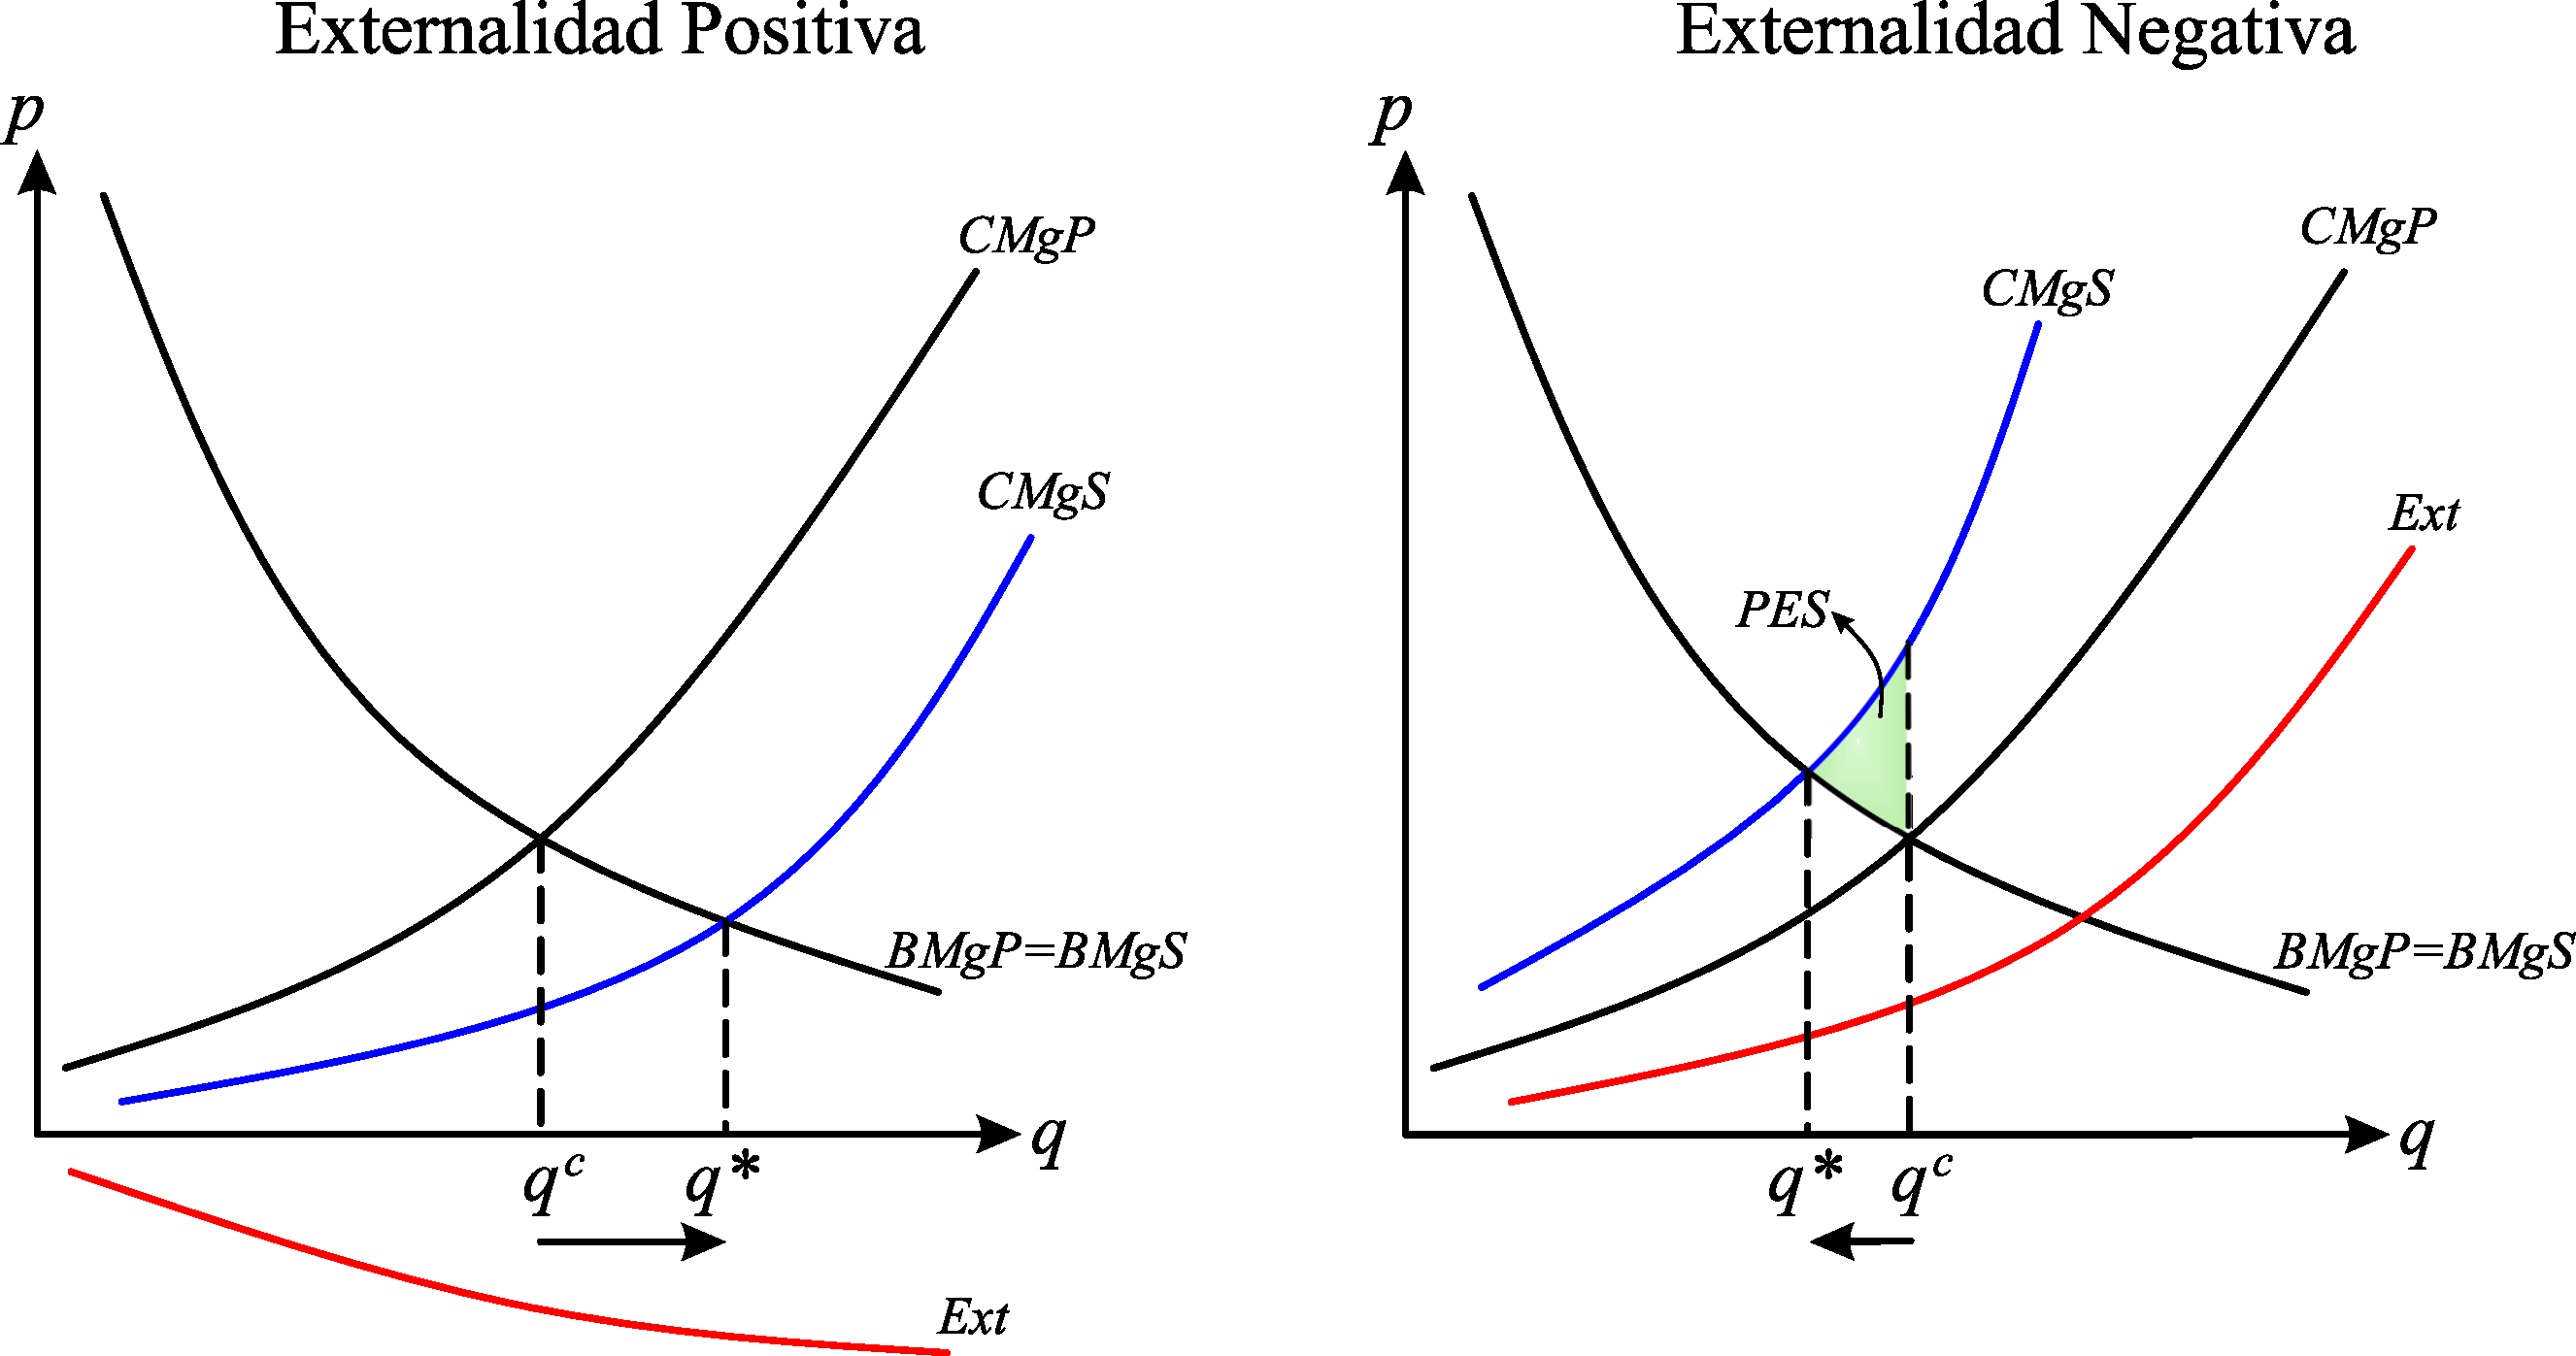
\includegraphics[width = 1\linewidth]{figures/produccion.pdf}
	\end{center}
\end{frame}
%------------------------------------------------
\begin{frame}{Externalidades de producción}
	\begin{itemize}
		\item Sean dos empresas: una acería $(S)$ y una piscigranja $(F)$.
		\item La empresa $S$ produce
			\begin{itemize}
				\item $s$ cantidad de acero
				\item $x$ cantidad de contaminación que se vierte a un río contiguo.
			\end{itemize}
		\item La empresa $F$ produce
			\begin{itemize}
				\item $f$ cantidad de pescado
			\end{itemize}
		\item La empresa $F$ se encuentra río abajo y se perjudica por la contaminación de la empresa $S$.
		\item Las funciones de costo son:
			\begin{itemize}
				\item Para S: $c_s(s,x)$
				\item Para F: $c_f(f,x)$
			\end{itemize}
	\end{itemize}
\end{frame}
%------------------------------------------------
\begin{frame}{Externalidades de producción}
	Supuestos
		\begin{itemize}
			\item La mayor contaminación eleva el costo de la producción de pescado
					$$\frac{\partial c_f}{\partial x} > 0$$
			\item La reducción del nivel de contaminación, elevará el costo de producción de acero
					$$\frac{\partial c_s}{\partial x} \leq 0$$
		\end{itemize}
\end{frame}
%------------------------------------------------
\begin{frame}{Problemas de maximización de beneficio}
	\begin{itemize}
		\item Para la acería: 
				$$\M \limits_{s,x} \pi_s = p_ss - c_s(s,x)$$
			  La acería elige la producción de acero y de contaminación que maximice su $\pi$.
		\item Para la piscigranja: 
				$$\M \limits_{f}\pi_f = p_f - c_f(f,x)$$
		      La piscigranja sólo determina cantidad de pescado, no controla la contaminación.
	\end{itemize}
\end{frame}
%------------------------------------------------
\begin{frame}{Problemas de maximización de beneficio}
	\begingroup
		\setlength{\tabcolsep}{10pt} % Default value: 6pt
		\renewcommand{\arraystretch}{1.5} % Default value: 1
			\begin{tabular}{ccc}
				\hline
					Para la acería & {} & Para la piscigranja\\
					$\M \limits_{s,x} \pi_s = p_ss - c_s(s,x)$ & {} & $\M \limits_{f} \pi_f = p_f - c_f(f,x)$\\
				\hline 
					\multicolumn{3}{c}{condiciones de primer orden} \\
				\hline
					$\frac{\partial \pi}{\partial s} = 0 \Leftrightarrow p_s - \frac{\partial c_s(s^\ast,x^\ast)}{\partial s} = 0$ & {} & $\frac{\partial \pi}{\partial f} = 0 \Leftrightarrow p_f - \frac{\partial c_f(f^\ast,x^\ast)}{\partial f} = 0$\\
					$p_s = \frac{\partial c_s(s^\ast,x^\ast)}{\partial s}$ & {} & $p_f = \frac{\partial c_f(f^\ast,x^\ast)}{\partial f}$\\
					$\frac{\partial \pi}{\partial x} = 0 \Leftrightarrow - \frac{\partial c_s(s^\ast,x^\ast)}{\partial x} = 0$ &{} & {}\\
					$0 = \frac{\partial c_s(s^\ast,x^\ast)}{\partial x}$& {} & {} \\
				\hline
			\end{tabular}
	\endgroup
\end{frame}
%------------------------------------------------
\begin{frame}{Problemas de maximización de beneficio}
	Interpretación
		\begin{itemize}
			\item La acería produce acero donde precio = $CMg$ de producir dicho acero.
					$$p_s = \frac{\partial c_s(s^\ast,x^\ast)}{\partial s}$$
			\item Y genera desechos donde el $CMg$ de producirlos es nulo.
					$$0 = \frac{\partial c_s(s^\ast,x^\ast)}{\partial x}$$
			\item La piscifactoría produce donde precio de pescado = CMg de producir pescado.
					$$p_f = \frac{\partial c_f(f^\ast,x^\ast)}{\partial f}$$
		\end{itemize}
\end{frame}
%------------------------------------------------
\begin{frame}{¿Por qué hay externalidad?}
	\begin{itemize}
		\item La acería produce demasiada contaminación, porque no le cuesta hacerlo.
		\item La cantidad óptima de acero sólo considera su costo de producción, no el daño que ocasiona a la piscigranja. 
		\item Como la piscigranja no puede controlar la cantidad de desecho que genera la acería, debe incurrir en mayores costos para eliminar el desecho del agua.
	\end{itemize}
\end{frame}
%------------------------------------------------
\begin{frame}{La solución eficiente}
	Fusionarse y maximizar el beneficio conjunto:
			$$\pi_s + \pi_f = p_ss - c_s(s,x) + p_ff - c_f(f,x)$$
				\vspace{-0.4cm}
		\begin{itemize}
			\item La empresa conjunta tiene en cuenta ahora los costos de todos los agentes ( costos de la producción de acero +  daño que le produce a la piscicultura). 
			\item Si: 
					$$\pi = p_ss + p_ff - c_s(s,x) - c_f(f,x)$$
			\item Las CPO son:
					\begin{gather*}
						\frac{\partial \pi}{\partial s} = 0 \Leftrightarrow p_s - \frac{\partial c_s(s^\ast,x^\ast)}{\partial s} = 0 \Leftrightarrow p_s - \frac{\partial c_S}{\partial s} - \frac{\partial c_f}{\partial x} \cdot \frac{\partial x}{\partial s} = 0\\
						p_s =  \frac{\partial c_s}{\partial s} + \frac{\partial c_f}{\partial x} \cdot \frac{\partial x}{\partial s}
					\end{gather*}
		\end{itemize}
\end{frame}
%------------------------------------------------
\begin{frame}{Gráficamente}
Por tanto, la producción óptima social de acero será menor a la producción privada.
	\begin{center}
		\begin{tikzpicture}[scale=1]
	% Formación de la caja
	% Consumidor A
	\draw[->] (0.5,0.5) node[align=center, below left] {\footnotesize $O_A$} -- (0.5,4.5) node[align=center, above] {\footnotesize $x_{2}^{A}$};
	\draw[->] (0.5,0.5) -- (8.5,0.5) node[align=center, right] {\footnotesize $x_{1}^{A}$};
	
	\draw (6,0.5) node[below] {\footnotesize $x_{1}^{A}$};
	\draw (0.5,2) node[left] {\footnotesize $x_{2}^{A}$};
	
	% Llaves
	\draw [decorate,decoration={brace,amplitude=5pt},xshift=-4pt,yshift=0pt] (6.1,-0.05) -- (0.7,-0.05);
	\node [right] at (3,-0.4) {$w_{1}^{A}$};
	
	\draw [decorate,decoration={brace,amplitude=5pt},xshift=-4pt,yshift=0pt] (-0.05,0.5) --(-0.05,2);
	\node [left] at (-0.3,1.27) {$w_{2}^{A}$};
\end{tikzpicture}
	\end{center}
\end{frame}
%------------------------------------------------
\begin{frame}{La solución eficiente}
	\begin{center}
		\begingroup
		\setlength{\tabcolsep}{10pt} % Default value: 6pt
		\renewcommand{\arraystretch}{1.5} % Default value: 1
			\begin{tabular}{p{4cm}cp{4cm}}
				\hline
					\multicolumn{3}{c}{Si: $\pi= p_ss + p_ff - c_s(s,x) - c_f(f,x)$} \\
				\hline
					Las CPO son: &{}&\\
				\hline
					$\frac{\partial \pi}{\partial x} = 0 \Leftrightarrow -\frac{\partial c_S}{\partial x} - \frac{\partial c_f}{\partial x} = 0$ &{}& $\frac{\partial \pi}{\partial f} \Leftrightarrow p_f - \frac{\partial c_f}{\partial f} = 0$\\
					$-\frac{\partial c_s}{\partial x} = \frac{\partial c_f}{\partial x}$ &{}& $p_f = \frac{\partial c_f}{\partial f}$\\
					&{}& Como la actividad de la piscigranja no ejerce externalidad, el óptimo privado es igual al óptimo social. \\
				\hline
			\end{tabular}
		\endgroup
	\end{center}
\end{frame}
%------------------------------------------------
\begin{frame}{Gráficamente}
La acería producirá menos desecho que antes porque enfrenta un costo positivo al contaminar, frente al costo nulo de antes.
	\begin{center}
		\vspace{-0.5cm}
\begin{tikzpicture}[scale=1.2]
	\hspace{-0.3cm}
	% Curva de contrato 5.2,2
		\draw  [purple, very thick] (0.5,0.5) ..controls (2,1.5) and (4.8,0) .. (5.2,2) ..controls (5.6,4.2) and (6.8,2.8) .. (8,4);
	% Intersección de una dotación
		% Oferta: w
			\draw[dashed, opacity=0.4] (6,4) node [above, opacity=1] {\footnotesize $w_{1}^{B}$} -- (6,0.5) node [below, opacity=1] {\footnotesize $w_{1}^{A}$};
			\draw[dashed, opacity=0.4] (0.5,1.62)  node [left, opacity=1] {\footnotesize $w_{2}^{A}$} -- (8,1.62) node [right, opacity=1] {\footnotesize $w_{2}^{B}$};
	
	% Curvas de indiferencia
		\draw [blue] (3.5,4) .. controls (4.6,2) and (5.2,1.7) .. (8,1.4);
		\draw [red] (0.5,2.7) .. controls (4.915,2.515) and (5.915,2.015) .. (6.5,0.5);
	
	% Recta presupuestaria
		\draw (0.5,4.23) -- (8.36,0.5);
		\draw [cyan](5.32,4) -- (6.32,0.5);
		
	% Flecha y rectángulo
		\draw [->] (2.48,3.29) -- (2.67,3.69) node [left, scale = 0.3mm] {\footnotesize $p$};
		\draw [rotate around={-25:(2.48,3.29)}] (2.48,3.29) rectangle (2.6, 3.4);
	
	% Puntos
		\draw[black, fill=black] (5.6,3.02) circle[radius=0.05] node [above, scale=0.25mm] {$N$};
		\draw[black, fill=black] (6,1.62) circle[radius=0.05] node [above right, scale=0.25mm] {$W$};
	
	% Formación de la caja
		% Consumidor A
			\draw[->] (0.5,0.5) node[align=center, below left] {\footnotesize $O_A$} -- (0.5,4.5) node[align=center, above] {\footnotesize $x_{2}^{A}$};
			\draw[->] (0.5,0.5) -- (8.5,0.5) node[align=center, right] {\footnotesize $x_{1}^{B}$};
			
		%Consumidor B
			\draw[->] (8,4) node[align=center, above right] {\footnotesize $O_B$} -- (0,4) node[align=center, left] {\footnotesize $x_{1}^{B}$};
			\draw[->] (8,4) -- (8,0) node[align=center, below] {\footnotesize $x_{2}^{B}$};
\end{tikzpicture}
	\end{center}
\end{frame}
%4) Aplicación al comercio internacional----------
	%====================================================================================
\section[Reconcimiento]{¿Cómo conseguir que las empresas reconozcan el costo social?}
%====================================================================================

\begin{frame}{¿Cómo conseguir que las empresas reconozcan el costo social?}
	\begin{itemize}
		\item Internalizar la externalidad (fusión del contaminante y el dañado).
		\item Impuestos / subsidios.
		\item Creación de mercados de derechos (Teorema de Coase)
	\end{itemize}
\end{frame}
%------------------------------------------------
\begin{frame}{Internalizar la externalidad:}
	\begin{itemize}
		\item Se da, por ejemplo, si la acería compra la empresa de piscicultura; por lo que le convendrá maximizar su producción de acero y minimizar el daño que esto le causa a la piscicultura.
		\item Este tipo de solución sólo es factible cuando hay pocos agentes.
	\end{itemize}
\end{frame}


%------------------------------------------------------------------------------------
% End
%----
	\begin{frame}
		\maketitle
		{\small
			\LaTeX \enskip support and edition:\\
			Joel Vicencio-Damian\\
			\vspace{-0.05cm}
			joel.nestor.damian@gmail.com \faIcon{envelope}}
	\end{frame}

%------------------------------------------------------------------------------------
\end{document}		
%====================================================================================